\begin{figure}[t]\centering
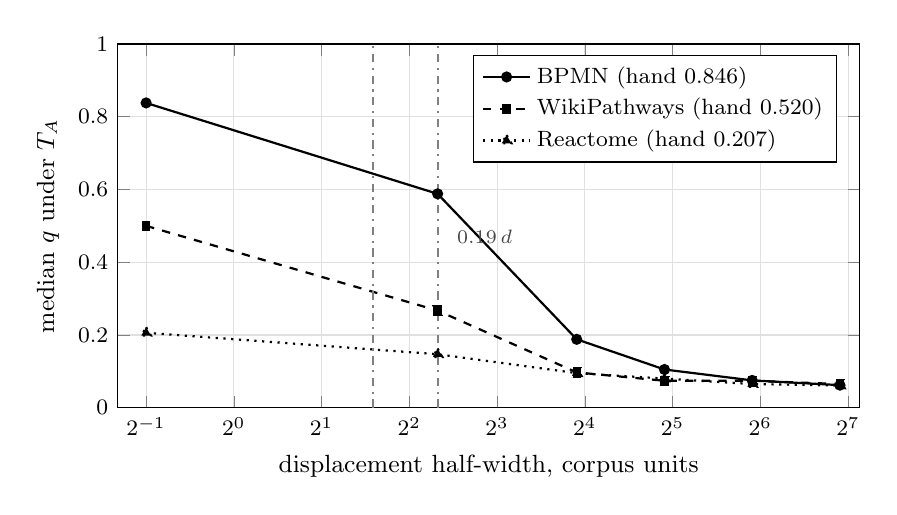
\begin{tikzpicture}
\begin{axis}[width=11cm,height=6.2cm,
  xmode=log,log basis x=2,
  xlabel={displacement half-width, corpus units},
  ylabel={median $q$ under $T_A$},
  ymin=0,ymax=1,xmin=0.4,xmax=140,
  legend pos=north east,legend cell align=left,
  grid=major,grid style={black!12},
  tick label style={font=\footnotesize},label style={font=\small},
  legend style={font=\footnotesize}]
\addplot[thick,mark=*,mark size=1.6pt] coordinates
  {(0.5,0.838)(5,0.588)(15,0.188)(30,0.105)(60,0.075)(120,0.062)};
\addlegendentry{BPMN (hand 0.846)}
\addplot[thick,mark=square*,mark size=1.5pt,dashed] coordinates
  {(0.5,0.500)(5,0.267)(15,0.097)(30,0.074)(60,0.074)(120,0.065)};
\addlegendentry{WikiPathways (hand 0.520)}
\addplot[thick,mark=triangle*,mark size=2pt,dotted] coordinates
  {(0.5,0.206)(5,0.147)(15,0.095)(30,0.080)(60,0.065)(120,0.061)};
\addlegendentry{Reactome (hand 0.207)}
\addplot[gray,thick,dash dot,forget plot] coordinates {(3,0)(3,1)};
\addplot[gray,thick,dash dot,forget plot] coordinates {(5,0)(5,1)};
\node[anchor=west,font=\scriptsize,gray!55!black] at (axis cs:5.4,0.47) {$0.19\,d$};
\end{axis}
\end{tikzpicture}
\caption{The displacement sweep, every box of every hand layout displaced by up to the
half-width, the alignment hold read at $d = 0.02$ and sixteen directions. The declared
half-pitch test sits at the left edge, 0.5 units, where nothing has changed: the corner of
$T_A$ releases a box only past $0.19\,d$, 3 units in the biological corpora and 5 in
BPMN. Past the bound the hold falls, BPMN 0.84 to 0.59 by a half-width of 5, and by 120
units every corpus is at the grid-snapped level of 0.06 to 0.09.}
\label{fig:sweep}
\end{figure}
